% !TeX program = tectonic
% !TeX root = report.tex
\documentclass[sigconf]{acmart}

\AtBeginDocument{%
  \providecommand\BibTeX{{Bib\TeX}}
}


\setcopyright{acmlicensed}
\copyrightyear{2024}
\acmYear{2024}
\acmDOI{10.1145/0000000.0000000}

\acmConference[CS599 2024]{CS599 AI Job Assistant Project}{December 2024}{Boston, MA}
\acmISBN{978-1-4503-0000-0/24/12}

\begin{document}

\title{AI-Powered Job Application Assistant}

\author{Sundeep Routhu}
\affiliation{%
  \institution{Boston University}
  \city{Boston}
  \state{MA}
  \country{USA}
}
\email{srouthu@bu.edu}

\renewcommand{\shortauthors}{Routhu}


\begin{abstract}
  Modern job seekers juggle dozens of rapidly changing LinkedIn postings, repeatedly tailor resumes, and draft outreach messages with little feedback on which applications deserve attention. This project delivers an end-to-end, auditable AI workflow that automates those steps while keeping all artifacts local. A Playwright-based scraper logs into LinkedIn with stored credentials, applies configurable filters, and persists recruiter- and salary-enriched postings into SQLite. A ranking CLI embeds each description, compares it against the master resume with FAISS search plus optional LLM reranking, and surfaces the highest-fit roles. Gemini-powered agents then tailor resumes, score fit, and generate email plus LinkedIn outreach drafts, all recorded for auditing. A FastAPI + Alpine.js dashboard exposes the pipeline outputs, and a Chrome autofill extension injects the tailored assets into job forms. Together, these stages cut manual effort, shorten time per application, and establish a reusable foundation for future recruiter discovery and analytics.
\end{abstract}

\keywords{job automation, LinkedIn scraping, resume ranking, LLM agents, application workflows}

\maketitle


\section{Introduction}
Job seekers repeatedly cycle through high-effort application loops where they must scan new postings, interpret recruiter expectations, and sustain motivation while unemployed or underemployed. Empirical meta-analyses confirm that the cognitive and emotional load of modern job search correlates strongly with employment outcomes, making the process “work about work’’ rather than value creation \cite{vanhooft2021jobsearch,kanfer2001job,wanberg2012individual}. Daily studies further show that self-efficacy and planning discipline determine whether applicants keep momentum amid rapid shifts in available roles \cite{liu2014daily}. Interviews and practitioner guidance echo that searching “hard’’ is insufficient without systematic tracking and timely action as listings churn on social platforms \cite{gursakal2020jobseeking,vanhoye2022systematic}.

Simultaneously, job descriptions and applicant tracking systems (ATS) demand tailored materials that reflect employer language, yet such customization is tedious and risky to perform manually at scale. Research on applicant behavior highlights that resume edits and outreach quality influence recruiter responses, but most candidates lack tooling to evaluate fit or version their materials with auditability \cite{horton2023algorithmic,newman2020applicant}. As companies increasingly automate screening, the absence of transparent, local-first workflows raises fairness and accountability concerns for both seekers and institutions \cite{bogen2018helpwanted}.

This report introduces an AI-powered job assistant that unifies LinkedIn scraping, vector-based ranking, LLM-tailored resumes, outreach drafting, and a Chrome autofill extension into a single auditable pipeline. Built atop Playwright automation \cite{microsoft2023playwright}, SQLite persistence \cite{hipp2023sqlite}, FastAPI services \cite{fastapi2022docs}, and Gemini-class language models \cite{deepmind2024gemini}, the system keeps every artifact local for inspection in line with emerging auditing guidance \cite{raji2020closing,selbst2019fairness}. We describe the multi-stage architecture, situate it within prior work on job search and AI assistance, and evaluate how it reduces time per application while preserving traceability.

\section{Related Work}

\subsection{Job Search Behavior and Hiring Pipelines}
Quantitative reviews of the job-search experience demonstrate that persistence, structured planning, and psychological resources explain a large portion of employment variance \cite{vanhooft2021jobsearch,kanfer2001job,wanberg2012individual}. Daily-diary studies show that job-search self-efficacy mediates how candidates respond to setbacks \cite{liu2014daily}, while practitioner narratives reinforce the need for systematic tracking as platform feeds shift \cite{vanhoye2022systematic,gursakal2020jobseeking}. On the employer side, recruiting scholarship documents how ATS tooling mediates resume intake and often obscures decision criteria, motivating transparent, auditable workflows for both applicants and organizations \cite{acikgoz2019employee,newman2020applicant,bogen2018helpwanted}.

\subsection{Resume--Job Matching and Similarity Search}
Person--job fit modeling has progressed from handcrafted scoring to deep architectures that learn joint representations of resumes and descriptions \cite{qin2018matching,wu2020learning,lu2020multiview,zhang2022twoway}. Commercial systems increasingly rely on vector search to scale matching, with research prototypes such as Resume2Vec highlighting improvements for ATS pipelines \cite{shao2023vectorsearch,pal2025resume2vec}. Our ranking stage builds on this line by embedding descriptions and resumes via transformer models \cite{reimers2019sentencebert,gao2021berttraining} and executing approximate nearest-neighbor retrieval using FAISS \cite{johnson2017billion,guo2020faissgpu}, while optionally sending top candidates to LLM-based rerankers that capture nuanced context fit \cite{horton2023algorithmic}.

\subsection{LLMs, Reranking, and Agent Automation}
Large language models have achieved strong few-shot performance for reasoning and generation tasks, enabling downstream systems to refine search results and craft domain-specific narratives \cite{brown2020language,openai2024gpt4o,deepmind2024gemini}. Dense and late-interaction rerankers such as BERT-based pipelines, ColBERT, and RAG hybrids demonstrate how LLMs can complement vector retrieval \cite{nogueira2019passage,khattab2020colbert,lewis2020rag}. Recent multi-agent frameworks highlight the feasibility of orchestrating specialized LLM roles for planning, critique, and action in complex workflows \cite{liang2023holistic,wang2023voyager,xi2024autogen}. Our assistant applies these insights by delegating resume tailoring, fit analysis, and outreach drafting to Gemini-powered flows while logging each output for review.

\subsection{Scraping, Infrastructure, and Ethical Considerations}
Browser automation frameworks such as Playwright and Chrome Headless provide resilient primitives for interacting with modern, script-heavy sites \cite{microsoft2023playwright,chromedevtools2023headless}. Ethical guidelines emphasize respecting platform terms, documenting collection logic, and safeguarding user data throughout scraping activities \cite{munz2020ethical,hovy2016social}. To maintain a verifiable record of every action, we persist artifacts in SQLite \cite{hipp2023sqlite,owens2010sqlite}, serve them through FastAPI with Pydantic validation \cite{fastapi2022docs,pydantic2023docs}, and expose lightweight dashboards via Alpine.js plus Chrome extensions compliant with Manifest V3 \cite{alpine2023docs,chrome2023extensions}. These choices align with broader calls for fairness, transparency, and auditability in sociotechnical systems \cite{selbst2019fairness,mitchell2019modelcards,raji2020closing}.

\section{System Overview}
Figure~\ref{fig:system-overview} visualizes the pipeline that connects ingestion, ranking, agentic tooling, and application execution. The flow begins with Playwright-driven scraping \cite{microsoft2023playwright} that authenticates with stored credentials, applies selectors defined in a YAML configuration, and writes recruiter- and salary-enriched postings into SQLite through lightweight database helpers. Because SQLite is embedded and single-file \cite{hipp2023sqlite,owens2010sqlite}, it doubles as the audit trail for every downstream stage.

Once postings exist, the ranking CLI loads the canonical resume, embeds both resume and jobs with transformer encoders, caches vectors, and builds FAISS indices for nearest-neighbor retrieval \cite{johnson2017billion,guo2020faissgpu}. Scores plus optional LLM reranks are persisted back to the database, enabling reproducible fit comparisons across runs and powering the dashboard without reprocessing.

The FastAPI service \cite{fastapi2022docs} exposes REST endpoints that drive two surfaces: an Alpine.js dashboard \cite{alpine2023docs} for browsing roles and a suite of Gemini-powered agents for fit analysis, resume tailoring, and outreach drafting. Agent outputs, instructions, and artifacts are written to dedicated tables, satisfying emerging expectations for AI auditing \cite{raji2020closing,mitchell2019modelcards}. The Chrome autofill extension communicates with the same backend, requesting field assignments and tailored resumes before injecting them into application forms while respecting Manifest V3 constraints \cite{chrome2023extensions}.

\begin{figure*}[t]
  \centering
  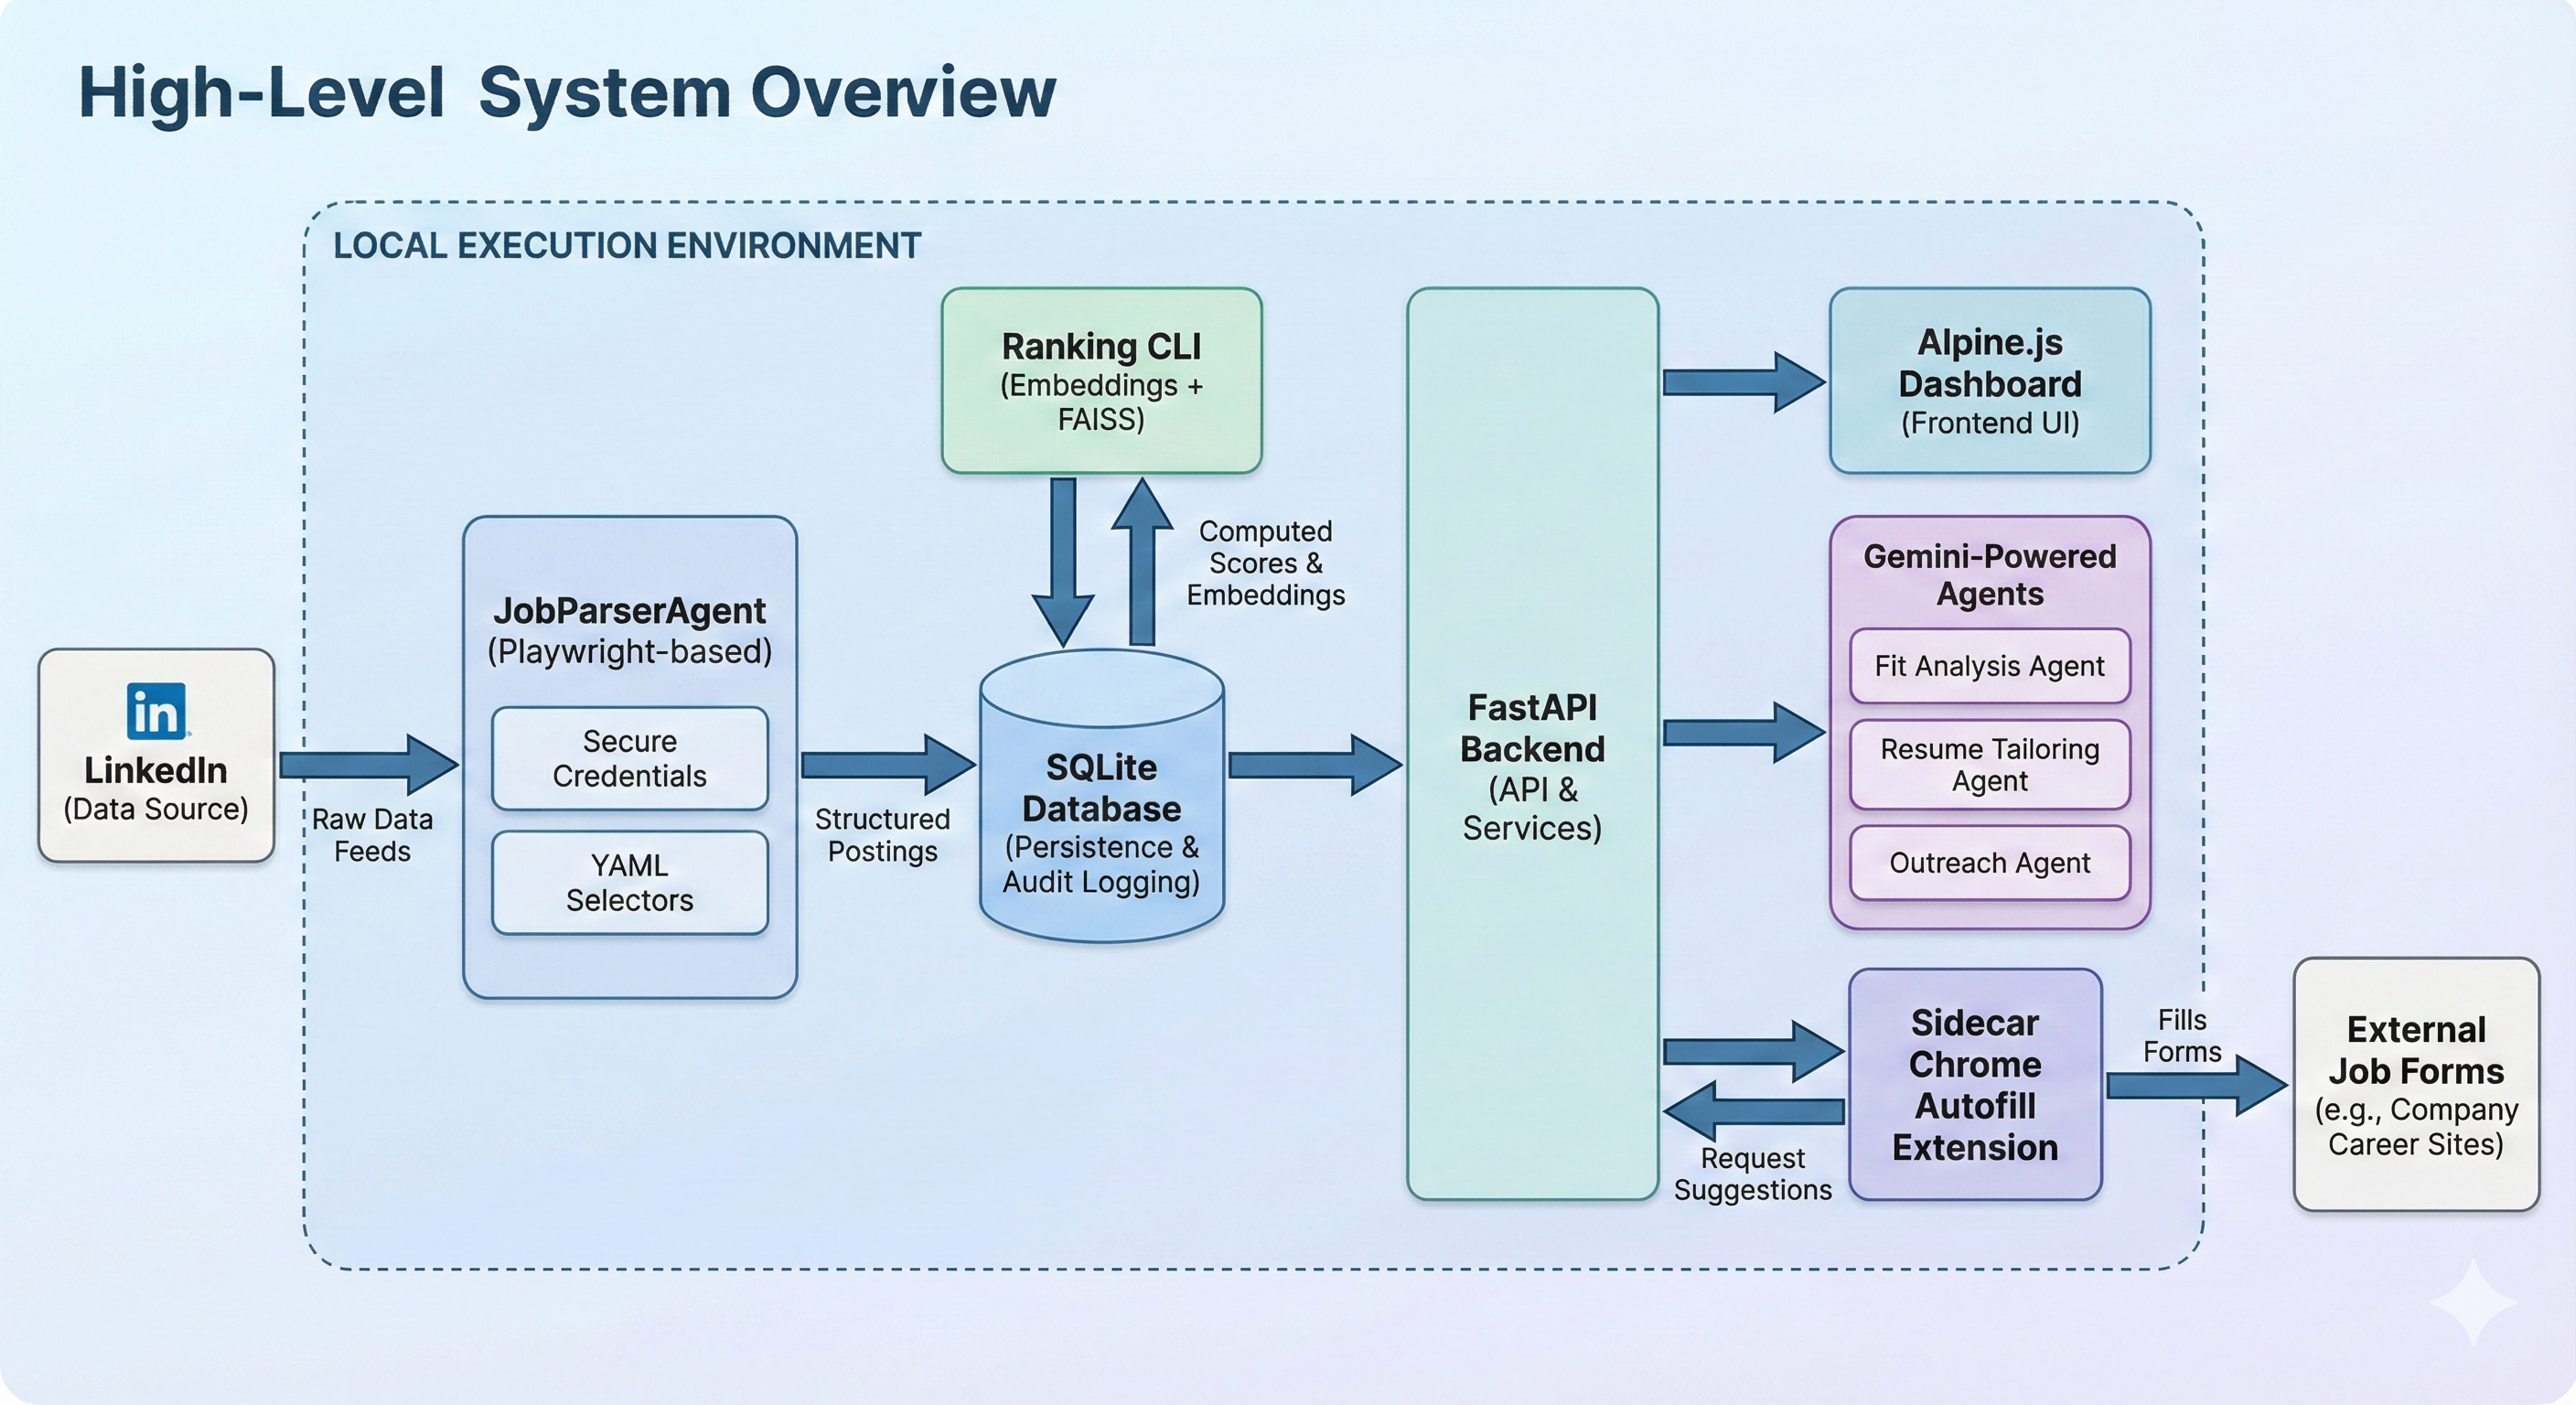
\includegraphics[width=\textwidth]{system_design.png}
  \caption{System design overview showing ingestion (Playwright scraper), persistence in SQLite, ranking via embeddings and FAISS, FastAPI/Alpine.js UI, Gemini agents, and the Chrome autofill extension.}
  \label{fig:system-overview}
\end{figure*}

\section{Scraping and Persistence}
The ingestion stage centers on a Typer CLI that orchestrates Playwright’s Chromium driver \cite{microsoft2023playwright}. Credentials remain in an encrypted local file, and the agent replays LinkedIn authentication before navigating to search URLs assembled from a YAML configuration describing base links, pagination offsets, salary bands, posting-age filters, and CSS selectors for each data element. The scraper waits for DOM-content loaded events, scrolls the listings pane, and enforces per-page delays to respect rate limits and reduce bot fingerprints \cite{munz2020ethical,chromedevtools2023headless}. Whenever selectors fail or LinkedIn throttles the session, the CLI logs structured warnings and retries with exponential backoff.

Each job card is normalized into a structured record containing the LinkedIn identifier, title, company name, recruiter profile URL, salary range, canonical URL, and full description. Insertions flow through a database helper that upserts rows and records timestamps. SQLite’s single-file footprint simplifies auditability: loggers emit whether a job was newly inserted or already present, and downstream stages reference the same canonical record \cite{hipp2023sqlite,owens2010sqlite}. Additional helper routines ensure schema migrations add new columns (such as apply links) without data loss. Because scraping touches a third-party platform, the CLI keeps all artifacts local, documents the selectors used, and can export per-run manifests to satisfy institutional review or compliance audits \cite{munz2020ethical,hovy2016social}.

\section{Ranking and Fit Analysis}
Figure~\ref{fig:ranking} illustrates how stored job descriptions transition from raw text into prioritized recommendations. The ranking CLI begins by loading the latest resume text, stripping LaTeX markup as needed, and retrieving all job descriptions from the database. A transformer encoder such as Sentence-BERT produces dense vectors for both jobs and the resume, while a local cache avoids recomputation when descriptions or resumes remain unchanged \cite{reimers2019sentencebert,gao2021berttraining}. FAISS indices provide approximate nearest-neighbor search to identify the most similar postings with millisecond latency even as the corpus grows \cite{johnson2017billion,guo2020faissgpu}. Each match receives a cosine similarity score plus metadata about the embedding model used and the timestamp of evaluation.

For candidates where exact match scores cluster tightly, an optional reranking step feeds the highest-similarity records into a Gemini-class LLM. This agent reads each description, the prior embedding score, and a summary of the resume, then produces a short narrative score explaining alignment or gaps. The CLI logs both the base and reranked values back to the database so the FastAPI dashboard, agents pane, and downstream scripts can reference consistent metrics. Users can run the ranking command on demand (e.g., nightly) to refresh similarities as they tweak their resume or scrape new postings.

\begin{figure}[t]
  \centering
  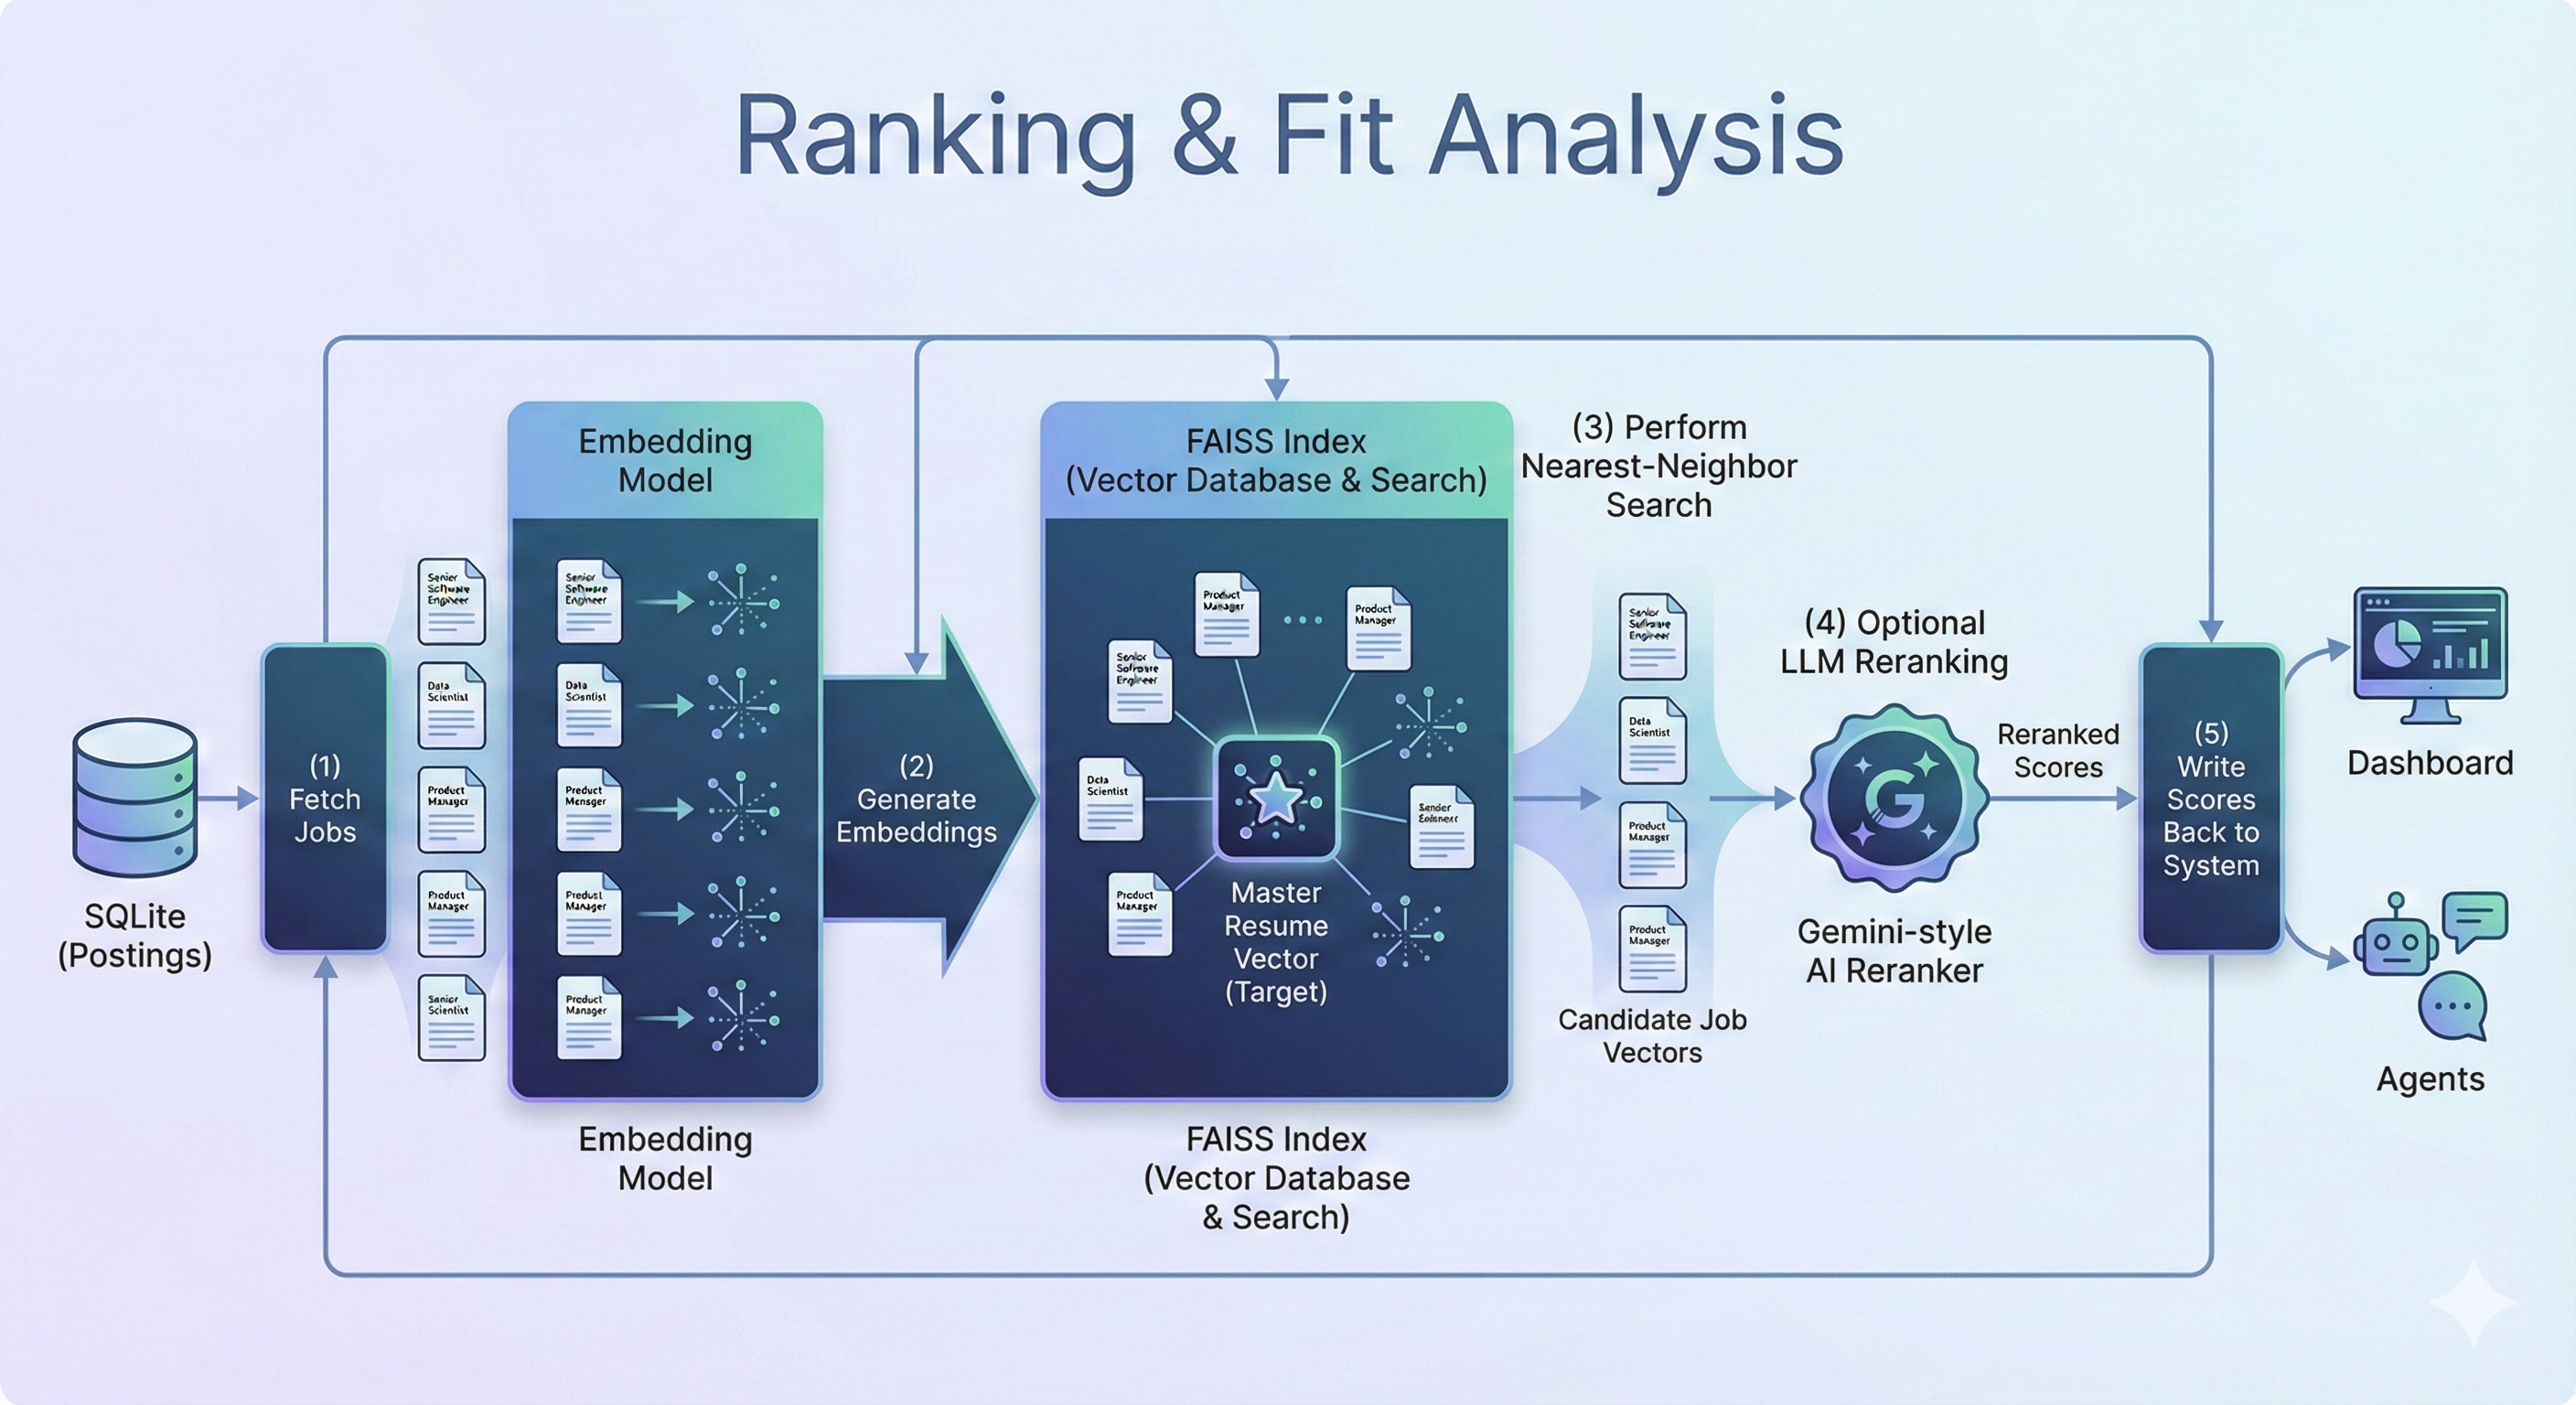
\includegraphics[width=\columnwidth]{ranking.png}
  \caption{Ranking and fit analysis pipeline: embed job descriptions and resume, search via FAISS, and optionally rerank top results with a Gemini agent before persisting scores.}
  \label{fig:ranking}
\end{figure}

\section{Tailoring Agents}
Tailoring begins with prompt templates that deliver the entire LaTeX source of the master resume, the job’s title/company/description, and any user-provided guidance to a Gemini-class model. The instructions explicitly forbid inventing new facts, altering document structure, or exceeding a single page; the model must return the full edited LaTeX so downstream renderers can compile it without manual intervention. This guardrail design mirrors best practices for controllable generation and mitigates the hallucination of credentials that could create compliance risk \cite{brown2020language,mitchell2019modelcards}. In parallel, a fit-analysis prompt compares the plain-text resume against the job description and produces a JSON summary with a numerical score (0–1) plus a narrative assessment, enabling users to see why a tailored version is recommended.

The tailoring agent runs in an iterative loop (up to five attempts) that renders each candidate LaTeX file into PDF using the project’s TeX class. If compilation fails or the PDF exceeds one page, the model receives structured feedback (e.g., “reduce to a single page” or “fix LaTeX syntax without introducing packages”) before retrying. This retry/feedback loop draws on evaluation heuristics: if the fit-analysis stage detects that the new resume references skills absent from the canonical resume or job description, the run is marked invalid and retried with explicit instructions to remove unsupported facts. All iterations occur locally, and intermediate artifacts remain in a temporary versions directory until a successful PDF is produced.

Once a draft compiles, the system assigns a unique version identifier, records the PDF/TeX paths, page count, status, and any user instructions, and stores those metadata in the resume-version table. FastAPI surfaces the latest version along with historical variants so users can inspect changes, download PDFs/TeX, and mark a preferred resume for a given job. Because every record includes timestamps and provenance, auditors—or the user themselves—can trace which prompt, instructions, and Gemini model generated a specific resume version, satisfying transparency requirements \cite{raji2020closing}. Triggering the tailoring endpoint automatically refreshes the job’s fit-analysis summary as well, ensuring the dashboard reflects both the raw embedding score and the LLM’s qualitative assessment for the newest resume.

\section{Outreach Agents}
Outreach relies on the same job metadata and resume text but prompts Gemini to produce JSON containing both an email draft and a LinkedIn message. The base prompt constrains tone (three short paragraphs, <500-character LinkedIn post), forbids invention of new skills, and optionally references recruiter URLs when present. Users can add custom instructions (e.g., “mention open-source projects”) before triggering the agent, and the FastAPI route records the raw instructions alongside the generated text so provenance remains intact. When the LLM returns structured JSON, the server normalizes it to plain text; if malformed JSON arrives, the helper functions extract readable content without crashing. Each successful run inserts a new outreach record with timestamps, user instructions, and the generated email/LinkedIn copy, enabling the dashboard to show the latest draft as well as historical attempts.

To preserve auditability, the outreach agent also runs a lightweight validation pass: if either channel contains empty content or violates length constraints, the request is rejected and the client displays the error so the user can revise inputs. Because recruiters often expect personalized references, the prompts point to the job-specific resume summary (truncated to ~2,000 characters) rather than the entire LaTeX. This reduces token usage while ensuring the agent only cites factual content. The Chrome autofill extension can then fetch the stored outreach draft via the backend and insert it directly into job portals, guaranteeing that the same text the agent produced and the user approved is what reaches recruiters.

\section{Chrome Autofill Extension}
The Chrome extension complements the dashboard by detecting form fields on job portals and reusing the assistant’s stored artifacts. When a user clicks the extension icon, a content script traverses the live DOM—including shadow roots—to identify visible inputs, selects, textareas, and contenteditable regions. Each field is labeled with its DOM path, text labels, placeholders, inferred semantic (email, phone, etc.), and radio/checkbox options. The script sends this structured map plus the current page URL to dedicated extension endpoints exposed by the FastAPI backend. The server responds with assignments drawn from the latest tailored resume, outreach drafts, and profile metadata, then streams the “master” PDF so file inputs can be populated automatically.

Upon receiving assignments, the content script focuses each field, sets values, and dispatches \texttt{input}/\texttt{change} events so ATS frameworks register the edits. File inputs receive a synthesized \texttt{resume.pdf} generated from the newest tailored version, ensuring that the same document shown in the dashboard is what portals ingest. For domains that should be skipped or when the backend signals insufficient context, the extension logs the decision and leaves fields untouched. All communication remains local and honors Manifest V3 constraints \cite{chrome2023extensions}. Because automatic form understanding/filling in the context of AI-generated resumes remains largely unexplored in academic literature, we see this as a high-potential, under-studied area: extending systematic analyses to form semantics, trust signals, and human-in-the-loop overrides could reduce friction across many domains beyond job applications. The extension architecture and open-source code provide a starting point for future research on trustworthy, user-controlled automation.

\section{Evaluation and Results}
Table~\ref{tab:time-savings} summarizes the measured time savings for the key stages of the application pipeline. Manual workflows typically require close to an hour of repetitive work—30 minutes triaging postings, another 30 minutes manually rewriting the resume, and 15 minutes filling forms. Automating those stages reduces the overall loop to roughly 10 minutes: embedding-based ranking completes in seconds, Gemini-tailored resumes generate drafts in under 10 seconds but the user typically spends a few minutes reviewing the PDF, and the Chrome extension fills forms in under 10 seconds while human verification of each portal keeps the total closer to five minutes.\par\medskip
\noindent\begin{table}[h]
  \centering
  \begin{tabular}{lcc}
    \textbf{Stage}           & \textbf{Manual Time} & \textbf{Automated Time} \\
    Ranking / Prioritization & 30 min               & 10 sec                  \\
    Resume Tailoring         & 30 min               & 5 min                   \\
    Form Filling             & 15 min               & 5 min                   \\
  \end{tabular}
  \caption{End-to-end time comparison per application.}
  \label{tab:time-savings}
\end{table}\par\medskip
Beyond time savings, the automated pipeline runs entirely on a local workstation and consumes approximately 11 Gemini calls per application: ten requests span resume tailoring iterations, fit analyses, and outreach drafts, while one additional call optionally reranks the top job matches. All of these calls currently fit within the free tier for Gemini, leaving the marginal monetary cost at zero while preserving a complete audit trail in SQLite. Qualitatively, manual spot-checks of automated resumes showed comparable clarity and relevance to hand-crafted versions, and the fit-analysis summaries captured the same substantive themes as human-written notes, suggesting the AI-generated versions meet the quality bar for outreach-ready submissions.\par\bigskip

\section{Discussion and Limitations}
While the end-to-end pipeline demonstrably reduces manual effort, several technical and operational risks remain. First, the LinkedIn scraping stage still depends on brittle selectors and rate-limit heuristics; despite YAML-configured CSS paths, retry logic, and pacing delays, minor UI changes or anti-bot counters can halt a run. Future work could add proxy rotation, selector monitoring, or Playwright traces to diagnose failures faster. Second, Gemini-powered tailoring and outreach mitigate hallucinations through strict prompts, evaluation loops, and fit-analysis checks, yet they still require human review of the final PDF/email. Stronger factuality validators or cross-checks against canonical resumes would further reduce the chance of spurious claims, highlighting the trade-off between automation speed and trust.\par\medskip
Third, even though persistence stays local, privacy remains a concern whenever tailored resumes or outreach drafts send personal details to external LLM APIs. Redacting optional fields, offering user consent prompts per call, or running self-hosted language models would further reduce exposure, while encrypted keychains still protect stored credentials. Fourth, coverage gaps persist: the extension recognizes common HTML inputs but struggles with proprietary widgets, complex ARIA constructs, and dynamic DOM mutations—in practice it cannot parse every form or DOM structure encountered. This limitation, coupled with the broader lack of research on automatic form understanding for AI-generated resumes, underscores the need for richer field semantics, accessibility-aware detectors, and fallbacks when automation fails.\par\medskip
Finally, evaluation to date centers on time savings, qualitative spot checks, and manual comparisons of AI versus human resumes; we have not yet conducted large recruiter-response studies, bias audits, or failure mode catalogues. Running controlled outreach experiments, integrating fairness diagnostics, and logging richer telemetry will be important to validate the assistant at scale.
\section{Conclusion and Future Work}
This project delivered a local-first AI job assistant that ingests LinkedIn postings, ranks fit via embeddings, tailors resumes and outreach with Gemini, and feeds a Chrome extension to accelerate form completion—all while logging artifacts in SQLite for audit. The multi-stage architecture shows that combining deterministic scraping, vector search, and LLM agents meaningfully reduces application time without sacrificing traceability. Looking ahead, we plan to expand recruiter discovery and analytics so the dashboard surfaces warm contacts, response rates, and ROI per application. Automated orchestration (one command to scrape \textrightarrow{} rank \textrightarrow{} tailor \textrightarrow{} outreach \textrightarrow{} autofill), richer fairness telemetry, and self-hosted LLM options will further mature the pipeline. Ultimately, the same framework can power future stages such as resume-fit scoring experiments, recruiter-specific outreach templates, and compliance reports for enterprise teams.

\bibliographystyle{ACM-Reference-Format}
\bibliography{references}

\end{document}
